\subsubsection{Search space}
\label{sec:bg:gp:repr_ev:space}
  Using this representation, we can define the \emph{genotype} of the
  individuals to contain only one \emph{chromosome} which is composed of a
  single \emph{gene}\footnote{%
    Although the most common representation is to have a single gene referencing
    the root of the tree, several variations that use multi-gene chromosomes
    have been proposed, such as Koza's \textit{Automatically Defined 
    Functions}~\autocite{kozaGeneticProgrammingII1994}, Angeline and Pollack's 
    \textit{Genetic Library Builder}~\autocite{peterjangelineEvolutionaryInductionSubroutines1992,peterj.angelineGeneticProgrammingEmergent1994},
    or Rosca and Ballard's \textit{Adaptive Representation}~\autocite{roscaLearningAdaptingRepresentations1994}.
  } that is the tree representation of the program.
  Recalling the definition of cardinality presented in
  \vref{def:cardinality_of_the_search_space}, we can see that the cardinality of
  the search space will be the number of possible trees that can be generated
  using the primitive set and the maximum height of the tree.

  \begin{lemma}
  \label{lemma:bg:gp:repr_ev:h_height_trees}
    Let \(\mathbb{T}_{H}\) be the set of all possible \textbf{labeled trees} of
    height \(H\), with \(H \in \mathbb{N}\).
    Given the sets \(\mathcal{T}\) and \(\mathcal{F}\) corresponding to the
    possible labels of terminal nodes (nodes that do not have children) and the
    possible labels of internal nodes (nodes that have children) respectively,
    the number of trees in \(\mathbb{T}_{H}\) is given by the following
    recurrence relation:

    \begin{equation}
      \label{eq:bg:gp:repr_ev:h_height_trees}
      |\mathbb{T}_{H}(\mathcal{T},\, \mathcal{F})| = \begin{cases}
        |\mathcal{T}| & \text{if } H = 0 \\
        \mathlarger{\sum}_{f \in \mathcal{F}} 
          |\mathbb{T}_{H-1}(\mathcal{T},\, \mathcal{F})|^{A(f)} 
          & \text{if } H > 0
      \end{cases}
    \end{equation}

    where \(A(f)\) is the arity of the node \(f\).
  \end{lemma}

  \begin{proof}
    For the proof, we will use induction on the height of the tree.
    For the sake of brevity, we will use the notation
    \(|\mathbb{T}_{H}(\mathcal{T},\, \mathcal{F})| = |\mathbb{T}_{H}|\).

    \paragraph{Base case: \(H = 0\)}
    If the height of the tree is 0, then the tree is composed of a single node,
    which is a terminal node.
    Thus, the number of possible trees is equal to the number of possible
    terminal nodes, which arises:

    \[
      |\mathbb{T}_{0}| = |\mathcal{T}|
    \]

    \paragraph{Base case: \(H = 1\)}
    If the height of the tree is 1, then the tree is composed of a root node,
    which is an internal node, and a set of children, which are terminal nodes.
    Suppose that the root node has the label \(f \in \mathcal{F}\) and arity
    \(A(f)\).
    
    Since the children are terminal nodes, each children can have any of the
    labels in \(\mathcal{T}\).
    Thus, the number of trees rooted at \(f\) is equal to the number of possible
    combinations of \(A(f)\) elements (with repetition and order) from the set
    \(\mathcal{T}\), this is:

    \[
      \prod_{i=1}^{A(f)} |\mathcal{T}| = |\mathcal{T}|^{A(f)}
    \]

    Since the root node can have any of the labels in \(\mathcal{F}\), the
    number of possible trees of height 1 is equal to:

    \[
      |\mathbb{T}_{1}| = \sum_{f \in \mathcal{F}} |\mathcal{T}|^{A(f)}
    \]

    \paragraph{Inductive step: \(H > 1\)}
    Suppose the statement holds true for \(H = h\).
    We aim to prove that the statement also holds true for \(H = h + 1\).

    Since a terminal node cannot have children,\footnote{
      This could also be interpreted as a terminal node having an arity of 0, or
      that all terminal nodes are leaves.
    } each tree of height \(h + 1\) has a root with one of the labels from the
    set \(\mathcal{F}\), and the remaining \(h\) layers are fully formed
    subtrees of height \(h\).

    For a given node label \(f \in \mathcal{F}\) with arity \(A(f)\), each child
    is the root of a subtree of height \(h\).
    Given our inductive assumption, there are \(|\mathbb{T}_{h}|\) possible
    such subtrees.

    Since all subtrees are independent, the number of possible trees with the
    root \(f\) is \(|\mathbb{T}_{h}|^{A(f)}\), which is the product of 
    \(|\mathbb{T}_{h}|\) over the arity of \(f\).

    We can sum this quantity over all \(f \in \mathcal{F}\) to get the total
    number of possible trees of height \(h + 1\):

    \[
      |\mathbb{T}_{h + 1}| = \sum_{f \in \mathcal{F}} |\mathbb{T}_{h}|^{A(f)}
    \]
  \end{proof}

  \begin{lemma}
  \label{lemma:bg:gp:repr_ev:leq_h_height_trees}
    Let \(\mathbb{T}_{\leq H}\) be the set of all possible \textbf{labeled 
    trees} of height \(h \leq H\), with \(H \in \mathbb{N}\) and \(h \in 
    \mathbb{N}\).
    Given the sets \(\mathcal{T}\) and \(\mathcal{F}\) corresponding to the
    possible labels of terminal nodes and the possible labels of internal nodes
    respectively, the number of trees in \(\mathbb{T}_{\leq H}\) is given by the
    following recurrence relation:

    \begin{equation}
      \label{eq:bg:gp:repr_ev:leq_h_height_trees}
      |\mathbb{T}_{\leq H}(\mathcal{T},\, \mathcal{F})| = \begin{cases}
        |\mathcal{T}| 
          & \text{if } H = 0 \\
        |\mathbb{T}_{H}(\mathcal{T},\, \mathcal{F})| 
            + |\mathbb{T}_{\leq H - 1}(\mathcal{T},\, \mathcal{F})|
          & \text{if } H > 0
      \end{cases}
    \end{equation}

    Where \(\mathbb{T}_{H}\) is the set of all possible trees of height \(H\).
  \end{lemma}

  \begin{proof}
    For the sake of simplicity, we will use the notation
    \(|\mathbb{T}_{\leq H}| = |\mathbb{T}_{\leq H}(\mathcal{T},\, \mathcal{F})|\)
    and \(|\mathbb{T}_{H}| = |\mathbb{T}_{H}(\mathcal{T},\, \mathcal{F})|\).

    The set \(\mathbb{T}_{\leq H}\) can be partitioned into two disjoint sets: 
    the set of all possible trees of height \(H\) and the set of all possible
    trees of height \(h < H\).
    Thus we have:
    
    \[
      |\mathbb{T}_{\leq H}| = |\mathbb{T}_{H}| + |\mathbb{T}_{\leq H - 1}|
    \]
  \end{proof}

  \begin{theorem}
  \label{thm:bg:gp:repr_ev:leq_h_height_trees}
    Let \(\mathbb{T}_{\leq H}\) be the set of all possible \textbf{labeled 
    trees} of height \(h \leq H\), with \(H \in \mathbb{N}\) and \(h \in 
    \mathbb{N}\).
    Given the sets \(\mathcal{T}\) and \(\mathcal{F}\) corresponding to the
    possible labels of terminal nodes and the possible labels of internal nodes 
    respectively, the number of trees in \(\mathbb{T}_{\leq H}\) is given by the
    following recurrence relation:

    \begin{equation}
      |\mathbb{T}_{\leq H}(\mathcal{T},\, \mathcal{F})| = \begin{cases}
        |\mathcal{T}| 
          & \text{if } H = 0 \\
        \left(\mathlarger{\sum}_{h = 0}^{H - 1}\,
          \mathlarger{\sum}_{f \in \mathcal{F}} 
            |\mathbb{T}_{h}(\mathcal{T},\, \mathcal{F})|^{A(f)}\right)
          + |\mathcal{T}|
          & \text{if } H > 0
      \end{cases}
    \end{equation}

    Where \(\mathbb{T}_{H}\) is the set of all possible trees of height \(H\) 
    and \(A(f)\) is the arity of the node \(f\).
  \end{theorem}

  \begin{proof}
    From \vref{lemma:bg:gp:repr_ev:leq_h_height_trees} we
    know the number of trees of height \(H\) or less is given by:

    \[
      |\mathbb{T}_{\leq H}| = |\mathbb{T}_{H}| + |\mathbb{T}_{\leq H - 1}|
    \]

    Then, by applying 
    \vref{lemma:bg:gp:repr_ev:h_height_trees}, we get:

    \[
      |\mathbb{T}_{\leq H}| = \left(\mathlarger{\sum}_{f \in \mathcal{F}} 
        |\mathbb{T}_{H - 1}|^{A(f)}\right) + |\mathbb{T}_{\leq H - 1}|
    \]

    By unrolling the recurrence relation, we get:

    \begin{align*}
      |\mathbb{T}_{\leq H}| 
        &= \left(
            \sum_{f \in \mathcal{F}} |\mathbb{T}_{H - 1}|^{A(f)}
          \right) + |\mathbb{T}_{\leq H - 1}| \\
        &= \left(
            \sum_{f \in \mathcal{F}} |\mathbb{T}_{H - 1}|^{A(f)}
          \right) + \left(
            \sum_{f \in \mathcal{F}} |\mathbb{T}_{H - 2}|^{A(f)}
          \right) + \cdots + \left(
            \sum_{f \in \mathcal{F}} |\mathbb{T}_{1}|^{A(f)}
          \right) + \left(
            \sum_{f \in \mathcal{F}} |\mathbb{T}_{0}|^{A(f)}
          \right) + |\mathbb{T}_{0}| \\
        &= \left(
          \sum_{h = 0}^{H - 1}\,
            \sum_{f \in \mathcal{F}} 
              \mathbb{T}_{h}(\mathcal{T},\, \mathcal{F})|^{A(f)}
          \right) + |\mathcal{T}|
    \end{align*}
  \end{proof}

  Given a program viewed as a \emph{labeled tree}, we can determine the 
  cardinality of the genetic programming algorithm's search space for a 
  specific maximum height \(H\). Considering the sets \(\mathcal{T} = \{x,\, 
  c\}\) and \(\mathcal{F} = \{+,\, -,\, \times,\, /,\, \sin,\, \cos,\, \exp,\, 
  \log\}\):

  \[
    A(f) = \begin{cases}
      2 & \text{for } f \in \{+,\, -,\, \times,\, /,\, \mathrm{pow}\} \\
      1 & \text{for } f \in \{\sin,\, \cos\}
    \end{cases}
  \]

  For an AST with a target program height of 4, we can set 5 as the maximum 
  height for the programs in our search space, offering some flexibility to the 
  generated programs. Given that \(c\) has 7 potential values, \(|\mathcal{T}| 
  = 8\), the search space's cardinality can be calculated accordingly.

  \begin{align*}
    |\mathcal{S}| 
      &= |\mathbb{T}_{\leq 5}(\mathcal{T},\, \mathcal{F})| 
        = \left(\mathlarger{\sum}_{h = 0}^{4}\,
          \mathlarger{\sum}_{f \in \mathcal{F}} 
          |\mathbb{T}_{h}(\mathcal{T},\, \mathcal{F})|^{A(f)}
        \right) + 8 \\
      &\approx 9.531\,142 \times 10^{37}  \\
      &\approx 10^{38}
  \end{align*}

  Thus, the search space of the genetic programming algorithm is of the order of
  \(10^{38}\) programs.\footnote{%
    This value was computed using the script shown in 
    \vref{lst:cardinality_of_T_leq_5}.
  }
  It should be easy to see that the size of the search space make it unfeasible
  to perform an exhaustive search.\footnote{If we approximate the time to
  evaluate a program to be 1 nanosecond, it would take approximately 3 sextillion years to evaluate all the programs in the search space.}

  This is why we need to use a heuristic search algorithm, such as genetic
  programming.
  In \vref{fig:bg:gp:repr_ev:leq_h_height_trees} we can see how the number of
  trees of height less or equal to \(h\) rapidly increases as \(h\) increases.

  \begin{figure}[ht!]
    \centering
    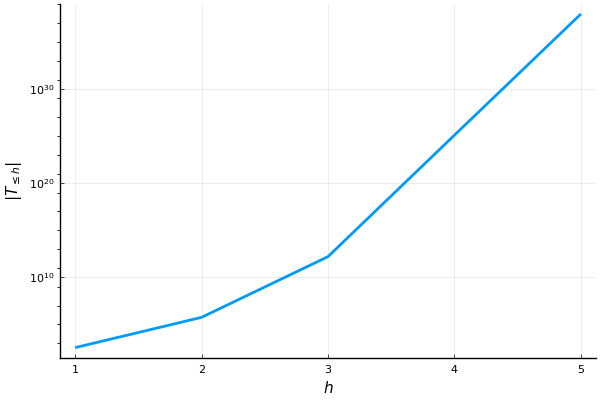
\includegraphics[width=0.5\textwidth]{img/theoretical_framework/t_leq.png}
    \caption{
      Total number of trees of height less or equal to \(h\) for \(h \in
      \{0,\, \ldots,\, 5\}\) and \(\mathcal{T} = \{x,\, c\}\) and \(\mathcal{F}
      = \{+,\, -,\, \times,\, /,\, \sin,\, \cos,\, \mathrm{pow}\}\).
      Note that the \(Y\) axis is in logarithmic scale.
    }
    \label{fig:bg:gp:repr_ev:leq_h_height_trees}
  \end{figure}